\chapter{Introduction}
\label{chap:intro}

\section{Background}
\label{s:intro_background}
Computer networks contain two types of elements: {\em end hosts} that generate
packets and {\em routers}\footnote{We use the term router to refer to both
switches and routers in this dissertation.} that forward these packets between
the end hosts. Historically, the Internet was architected so that most of the
complexity resided in the end hosts, while the routers themselves were simple.
According to Clark~\cite{design_philosophy}, this architecture was a result of
the primary design goal of the Internet: the ability to easily interconnect a
wide variety of existing networks (\eg long-haul networks, local-area networks,
satellite networks, and radio networks) through a set of routers
 between these networks. Quoting Clark, ``The Internet
architecture achieves this flexibility by making a minimum set of assumptions
about the function which the net will provide.''

The minimum functionality assumed of and provided by the network's routers was
best-effort and unreliable packet forwarding. Notably absent from a router's
feature set were reliable packet delivery, packet prioritization, monitoring
features to attribute a router's resource usage to specific end hosts, and
security features to detect network breaches. As a result, the early routers
were singularly dedicated to packet forwarding. A focus on packet forwarding
alone made it simpler to design high-speed routers. It also helped broaden the
Internet's reach by interconnecting existing networks with minimum friction.
But, it sidelined other goals~\cite{design_philosophy} such as network
performance, security, and monitoring.
 
Today, four decades after ideas underlying the Internet were first
published~\cite{cerf74}, it is clear that routers need to do much more than
packet forwarding for at least two reasons. First, once the basic goal of
interconnecting different networks is achieved, other goals like performance,
security, and monitoring rise in prominence.  Second, many large-scale private
networks (\eg datacenters, private wide-area networks, enterprise networks) do
not need to concern themselves with interconnecting diverse networks as the
Internet had to. Such private networks can expect more from the network. As a
result, a typical router today implements many features beyond packet
forwarding, pertaining to security (\eg access control), monitoring (\eg
counting the number of packets belonging to each flow), and performance (\eg
priority queues).

While a router's feature set has grown steadily with time, there's little
consensus between network operators and router vendors on a router's feature
set. Inevitably, there are network operators whose needs fall outside their
router's feature set. But because today's fastest routers are built out of
specialized forwarding hardware, they are largely {\em
fixed-function}\footnote{The term fixed-function was first used to describe
graphics processing units (GPUs) with limited or no
programmability~\cite{gpu_fixed}. We use it in an analogous sense here.}
devices, \ie their functionality cannot be changed once the router has been
built. In such cases, the operator has no alternative but to wait 2--3 years
for the next generation of the router hardware. This is best illustrated by the
lag time between the standardization and availability of new overlay
protocols~\cite{nvgre}.

As a result, the rate of innovation in new router algorithms is outstripping
our ability to get these algorithms into today's fastest routers. These routers
have between 10 and 100 ports, each running at between 10 and 100 Gbit/s, \ie
aggregate speeds in the several hundred Gbit/s to Tbit/s range.
Figure~\ref{fig:router_algos} shows a timeline of prominent router algorithms
that have been developed since the 1980s. Of these, only a handful are
available in the fastest routers today because there is no way to program a new
router algorithm on these routers.

\begin{figure}
\centering
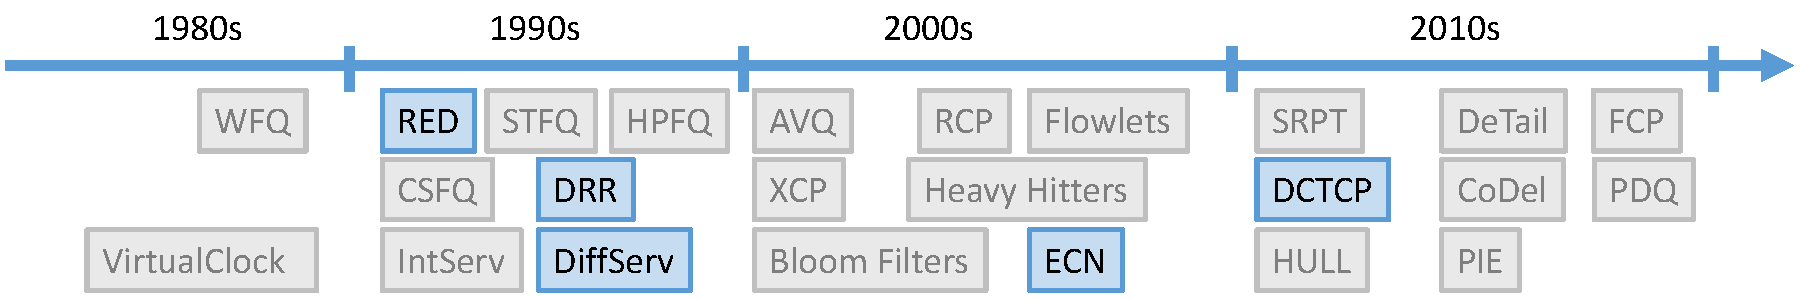
\includegraphics[width=\columnwidth]{router_alg_timeline.pdf}
\caption{Timeline of prominent router algorithms since the 1980s. Only the ones
shaded in blue are available on the fastest routers today.}
\label{fig:router_algos}
\end{figure}

For an operator wanting to introduce new functionality in their network, what
are the operator's choices? One is to give up on changing routers altogether
and make all the required changes at the end hosts.  Relying solely on the end
hosts, however, results in cumbersome or suboptimal solutions. As a first
example, imagine measuring the queueing latency at a particular hop in the
network. One could do this by collecting end-to-end ping measurements between a
variety of vantage points and then fusing these measurements together to
estimate per-hop queueing latency---a process commonly called network
tomography. Not only is this indirect, it is also inaccurate relatively to
directly instrumenting the router at that hop to measure its own queueing
latency. As a second example, consider the problem of congestion control, which
divides up a network's capacity fairly among competing users. There are many
in-network solutions to congestion control~\cite{xcp, rcp}, which outperform
the end-host-only approaches to congestion control used today~\cite{cubic,
compound}. However, there is no way to deploy these in-network solutions using
a fixed-function router today.
%TODO: find citation for tomography

Another alternative is to use a \textit{software router}: a catch-all term for
a router built on top of some programmable substrate, such as a general-purpose
CPU~\cite{click, routebricks}, a network processor\footnote{A CPU with an
instruction set tailored to packet processing~\cite{ixp4xx, ixp2800}.}, a
graphics processing unit (GPU)~\cite{packetshader}, or a field-programmable
gate array (FPGA)~\cite{netfpga}.  Figure~\ref{fig:router_evolution} tracks the
evolution of aggregate capacity of software routers and compares them to the
fastest routers known at any point in time. The figure shows two trends.
First, until the mid 1990s, software routers were in fact the fastest routers;
the early routers~\cite{imp} were minicomputers loaded with forwarding
software. Second, since the mid 1990s, growing demands for higher link speeds,
fueled by the Internet's growth, have meant that the fastest routers are now
built out of dedicated hardware.

Hardware specialization gives today's fastest routers a 10--100 $\times$ performance
improvement relative to the fastest software routers.  This performance improvement is the
result of fully exploiting the abundant parallelism available in packet
processing. First, data parallelism, the ability to simultaneously process
either different parts of the same packet or packets belonging to different
ports. Second, pipeline parallelism, the ability to simultaneously perform
different operations on different packets. But, hardware specialization carries
a cost: because routers are built out of specialized hardware, they are
fixed-function devices that can not be reconfigured or programmed in the field.

Recent work in software-defined networking~\cite{sdn_history} (SDN) and
programmable router chips~\cite{rmt, xpliant, flexpipe} has endowed fast
routers with limited flexibility. SDN allows operators to program the network's
control plane, which is the part of the network that computes a network's
routing tables. SDN does this by moving route computations out of the routers
and on to a logically centralized programmable server running on a CPU.

Programmable router chips allow operators to program parts of the data plane:
the part of the network that forwards packets based on the routing tables. For
instance, these chips allow an operator to program the router's parser to
recognize new packet headers, such as a new overlay format~\cite{nvgre}.
They also allow the operator to program packet header transformations (\eg
decrementing the IP TTL field) so long as these transformations do not modify
router state.

However, both SDN and programmable router chips are still insufficient to
express the grayed-out algorithms shown in Figure~\ref{fig:router_algos}
because (1) these algorithms programmatically manipulate router state and (2)
they require flexibility in packet scheduling.  State modification on routers
and the router's scheduler are largely ignored by both SDN and programmable
router chips.

\begin{figure}
\centering
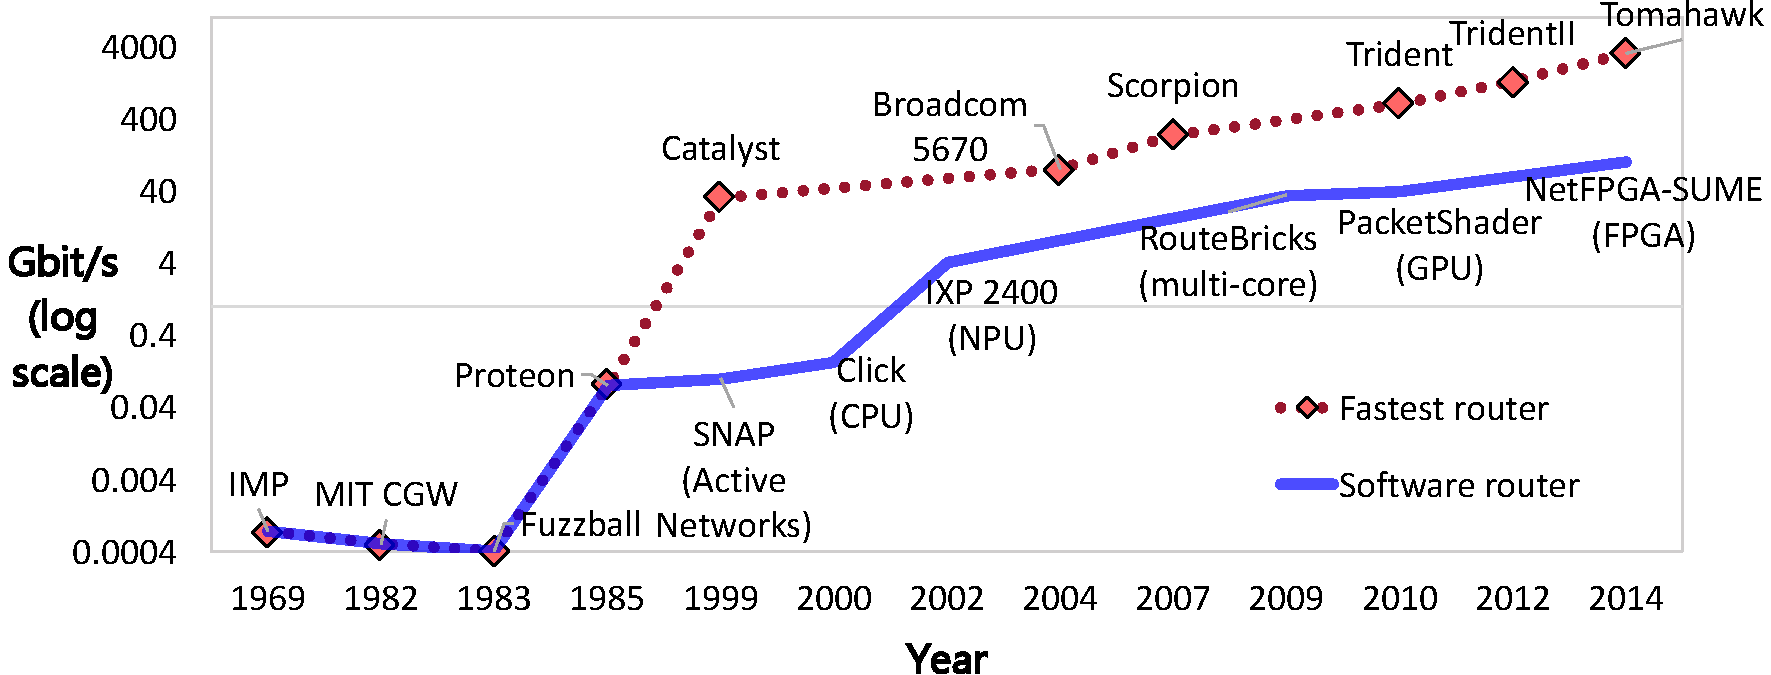
\includegraphics[width=\columnwidth]{router_evolution.pdf}
\caption{Aggregate capacity of software routers since the first router on the
ARPANET in 1969~\cite{imp}. Until the mid 1990s, software routers were
sufficient. Since then, however, the fastest routers have largely been
fixed-function devices, built out of dedicated non-programmable hardware, which
gives these routers a 10--100x performance improvement relative to the best
software routers.}
\label{fig:router_evolution}
\end{figure}

\section{Primary contributions}
\begin{table}
\textbf{Stateful data-plane algorithms (Chapter~\ref{chap:domino})}
\\[-7pt]\rule{\textwidth}{1pt}\\[-7pt]\rule{\textwidth}{1pt} \\
\textbf{Examples:} In-network congestion control (\eg XCP~\cite{xcp} and
RCP~\cite{rcp}), active queue management (\eg RED~\cite{red}, BLUE~\cite{blue},
and CoDel~\cite{codel}) \\
\textbf{Technical challenge:} How do we allow programmable router state
modification at the router's line rate, when a new packet can be received as
often as every nanosecond? \\
\textbf{Programming model:} Packet transactions (\S\ref{s:transactions})\\
\textbf{Hardware primitive:} Atoms (\S\ref{s:absmachine}) \\
\textbf{Key finding:} A small set of atoms (Table~\ref{tab:templates}) is
simultaneously (1) expressive enough to serve as the instruction set for many
stateful algorithms (Table~\ref{tab:algo_atoms}) and (2) feasible
in high-speed hardware (\S\ref{s:eval}). Further, we find that these atoms
can support several new use cases that were unanticipated at the time the atoms
were designed (Table~\ref{tab:atoms_generalize}).\\ \\

\textbf{Scheduling algorithms (Chapter~\ref{chap:pifo})}
\\[-7pt]\rule{\textwidth}{1pt}\\[-7pt]\rule{\textwidth}{1pt} \\
\textbf{Examples:} Weighted Fair Queueing~\cite{wfq} and priority scheduling~\cite{srpt} \\
\textbf{Technical challenge:} Can we find an abstraction that unifies many disparate
scheduling algorithms? \\
\textbf{Programming model:} Scheduling trees (\S\ref{s:pifo}) \\
\textbf{Hardware primitive:} A priority queue data structure called a Push In First Out
Queue (PIFO) (\S\ref{s:design}) \\
\textbf{Key finding:} A priority queue of packets with a program to set each
packet's priority can express many scheduling algorithms
(\S\ref{s:expressive}) and is feasible in high-speed hardware
(\S\ref{s:hardware}). \\\\

\textbf{Scalable per-flow statistics (Chapter~\ref{chap:perf_query})}
\\[-7pt]\rule{\textwidth}{1pt}\\[-7pt]\rule{\textwidth}{1pt} \\
\textbf{Examples:} Per-flow measurements of moving averages, counters, and loss rates \\
\textbf{Technical challenge:} Can we allow programmers to flexibly define the
per-flow statistics they want to measure and also scale these measurements to a large number of
flows?\\
\textbf{Programming model:} Performance queries (\S\ref{sec:language}) \\
\textbf{Hardware primitive:} Programmable hardware key-value store. Keys correspond to
flows and values to statistics. (\S\ref{sec:aggregation}) \\
\textbf{Key finding:} A class of statistics measurements, which we call the
linear-in-state class (\S\ref{sec:linear-in-state-description}), can be scaled
to a large number of flows without losing accuracy. This class covers many
practically useful statistics such as counters, moving average filters, and
conditional counters (\S\ref{sec:eval}). \\
\caption{Contributions of this dissertation}
\label{tab:contributions}
\end{table}


This dissertation considers the problem of designing routers that approach the
speeds of today's fastest fixed-function routers, while also being
programmable. My thesis is that {\em it is possible to design router hardware
that is both fast and programmable, if we restrict ourselves to programming
specific classes of router functionality}. It is this specificity that allows
us to resolve the programmability-performance tension; indeed, our designs
provide a much more restricted form of programmability than a Turing-complete
processor.  The challenge here is to pick classes of router functionality that
are simultaneously (1) practically useful to network operators, (2) broad
enough to cover a range of current and future use cases within that class, and
yet (3) narrowly focused enough to permit a high-speed hardware implementation.
We will describe high-speed programmable hardware primitives and their
corresponding programming models in software for three classes of router
functionality: stateful data-plane algorithms, packet scheduling, and scalable
network measurement.  Table~\ref{tab:contributions} summarizes our
contributions.

\subsection{Evaluation metrics}
\label{ss:eval_metrics}

The goal of this dissertation is to design fast and programmable routers.
Accordingly, we measure each of our three systems on two attributes,
performance and programmability, as described below.

The traditional approach to evaluating performance of a software system is to
measure the system's throughput on some workloads. This approach does not apply
to evaluating hardware designs, which are built for a specific clock rate or
throughput. Hardware designs provide this clock rate or throughput even under
worst-case conditions, regardless of the workload presented to them. To provide
worst-case guarantees, hardware designs exploit spatial parallelism---by
chaining together computations in a pipeline (pipeline parallelism) and
simultaneously performing multiple operations within a pipeline stage (data
parallelism).  Put differently, hardware designs spend circuit area in return
for deterministic  high performance. The question then is whether these designs
consume a large amount of area to provide such performance guarantees and
whether they can provide an acceptable clock rate.
 
Hence, to evaluate performance, we estimate if the hardware components of our
systems can run at a high clock rate while not taking up too much gate and wire
area. To do so, we code up any new hardware components as programs in the
Verilog hardware description language.  We then pass this Verilog program to a
logic synthesis tool~\cite{synopsys_dc, cadence_rc} that produces a gate-level
implementation from Verilog programs.  The synthesis tool also reports whether
the resulting implementation meets timing at a given clock frequency and the
area taken up by the gates in the implementation.\footnote{A full hardware
implementation also requires a place-and-route~\cite{par} step after logic
synthesis to physically place these gates and route wires between them. This
increases the area of designs, especially if the design is dominated by wires,
as is the case with crossbars. Because our designs are dominated by gates, not
wires, we do not perform this place-and-route step when estimating area.} When
we say a hardware design is feasible, we mean that it meets timing at a high
clock frequency (1 GHz in this dissertation) and its gate area is modest
relative to the area of a router chip (200 \si{\milli\meter\squared} based on
the minimum area estimates provided by Gibb et al.~\cite{gibb_parsing}). 

To evaluate if our systems are programmable, we evaluate the expressiveness of
the programming models in each of our system. If we are able to express a
diversity of algorithms using the programming models, we say that the
programming model is expressive. Our approach to expressiveness is empirical:
beyond specific examples, we do not yet have theoretical characterizations of
the set of programs that can or cannot be programmed using our programming
models (\S\ref{ss:limit_completeness}).

In addition, to assess the correctness of our designs, we built a C++ simulator
of a programmable router that models the behavior of the essential
computational elements of a programmable router at the level of individual
clock cycles (\S\ref{s:absmachine}).

\section{Stateful data-plane algorithms}
In Chapter~\ref{chap:domino}), we consider the problem of programming {\em
stateful data-plane algorithms} at high packet processing rates. These are
algorithms that operate on a sequence of packets in a streaming manner, doing
a bounded amount of work per packet and manipulating a bounded amount of router
state in the process.  They include algorithms for managing the router's buffer
(\eg RED~\cite{red} and BLUE~\cite{blue}), load balancing (\eg
CONGA~\cite{conga} and flowlet switching~\cite{flowlets}), and in-network
congestion control (\eg XCP~\cite{xcp} and RCP~\cite{rcp}).

High-speed data-plane programming on routers poses two challenges: (1) what hardware
instructions are required to support programmable state modification at high
speeds, and (2) what is the right programming model? To address these
challenges, we develop a system for data-plane programming, Domino, which
contains three main components: an instruction set (atoms), a programming model
(packet transactions), and a compiler from packet transactions to atoms.

\subsection{Atoms: Hardware for high-speed state manipulation}
\label{ss:intro_atoms}
\textit{Atoms} capture a router's instruction set. They specify atomic units of
packet processing provided by the router hardware, \eg an atomic counter or an
atomic test-and-set. Figure~\ref{fig:simple_atom} shows an example atom. Atoms
are atomic in the sense that if some state is updated by an atom as part of
processing a packet, the next packet arriving at that atom will see the updated
value of that state. The processing within atoms is constrained to meet the
atomicity requirement. We enforce this constraint when designing atoms in
hardware by ensuring  that the input-to-output latency of the atom's digital
circuit is under a clock cycle. This guarantees that any state updated by the
atom has been updated to its correct value in time for the next packet arriving
at the atom a clock cycle later.\footnote{Note that this is a sufficient
condition for atomicity and may not always be necessary.}
%TODO: If I write out the multi-cycle atomics in concl.tex, I can reference that
%in the footnote.

\subsection{Packet transactions: A programming model for stateful algorithms}

\textit{Packet transactions} provide a
programming model for data-plane algorithms. A packet transaction is an atomic
and isolated block of code capturing an algorithm's logic written in a
domain-specific language (DSL) called Domino.
Figure~\ref{fig:simple_transaction} shows an example packet transaction.
Packet transactions provide programmers with the illusion that the
transaction's body executes serially from start to finish on each packet, in
the order in which packets arrive at the router. Conceptually, when programming
with packet transactions, there is no overlap in packet processing across
packets---akin to an infinitely fast single-threaded processor carrying out
packet processing on each packet. Packet transactions are expressive and
capture many important data-plane algorithms.  Further, their serial semantics
shield programmers from the router's data and pipeline parallelism.
%%Packet transactions have been
%%adopted in P4~\cite{p4}, a packet-processing language that is emerging as an
%%industry standard for programming router chips.  P4 programmers can now use an
%%@atomic annotation around a block of statements to specify that the block must
%%execute atomically.

\begin{figure}[!t]
\begin{minipage}{0.48\textwidth}
\centering
\vspace{0.38in}
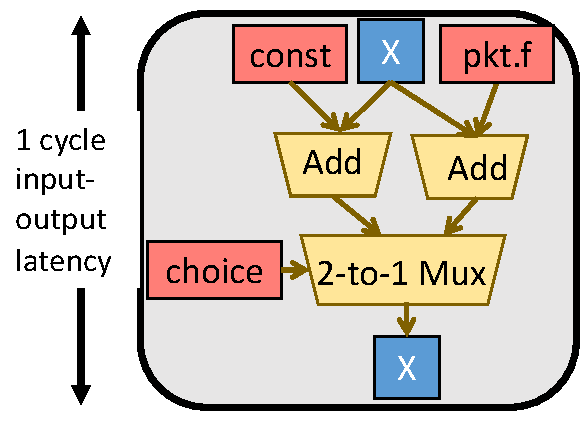
\includegraphics[width=0.85\textwidth]{atom.pdf}
\caption{An atom that either adds either a constant or a packet field to a
piece of state x and writes it back to x.}
\label{fig:simple_atom}
\end{minipage}
\hfill
\begin{minipage}{0.48\textwidth}
\centering
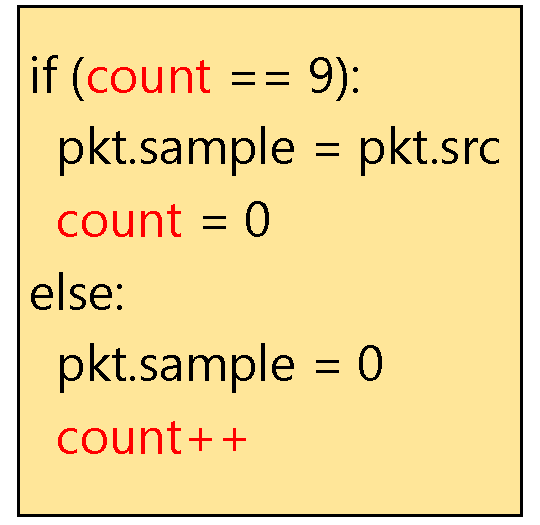
\includegraphics[width=0.75\textwidth]{packet_transaction.pdf}
\caption{A packet transaction that samples the source IP address of every 10th
packet. State variables (count) are in red.}
\label{fig:simple_transaction}
\end{minipage}
\end{figure}

\subsection{Compiling from packet transactions to atoms}
The Domino compiler compiles packet transactions
written in the Domino DSL to a pipeline of atoms provided by the router. It
rejects the code if the router's atoms cannot support the packet transaction.

\begin{figure}[!t]
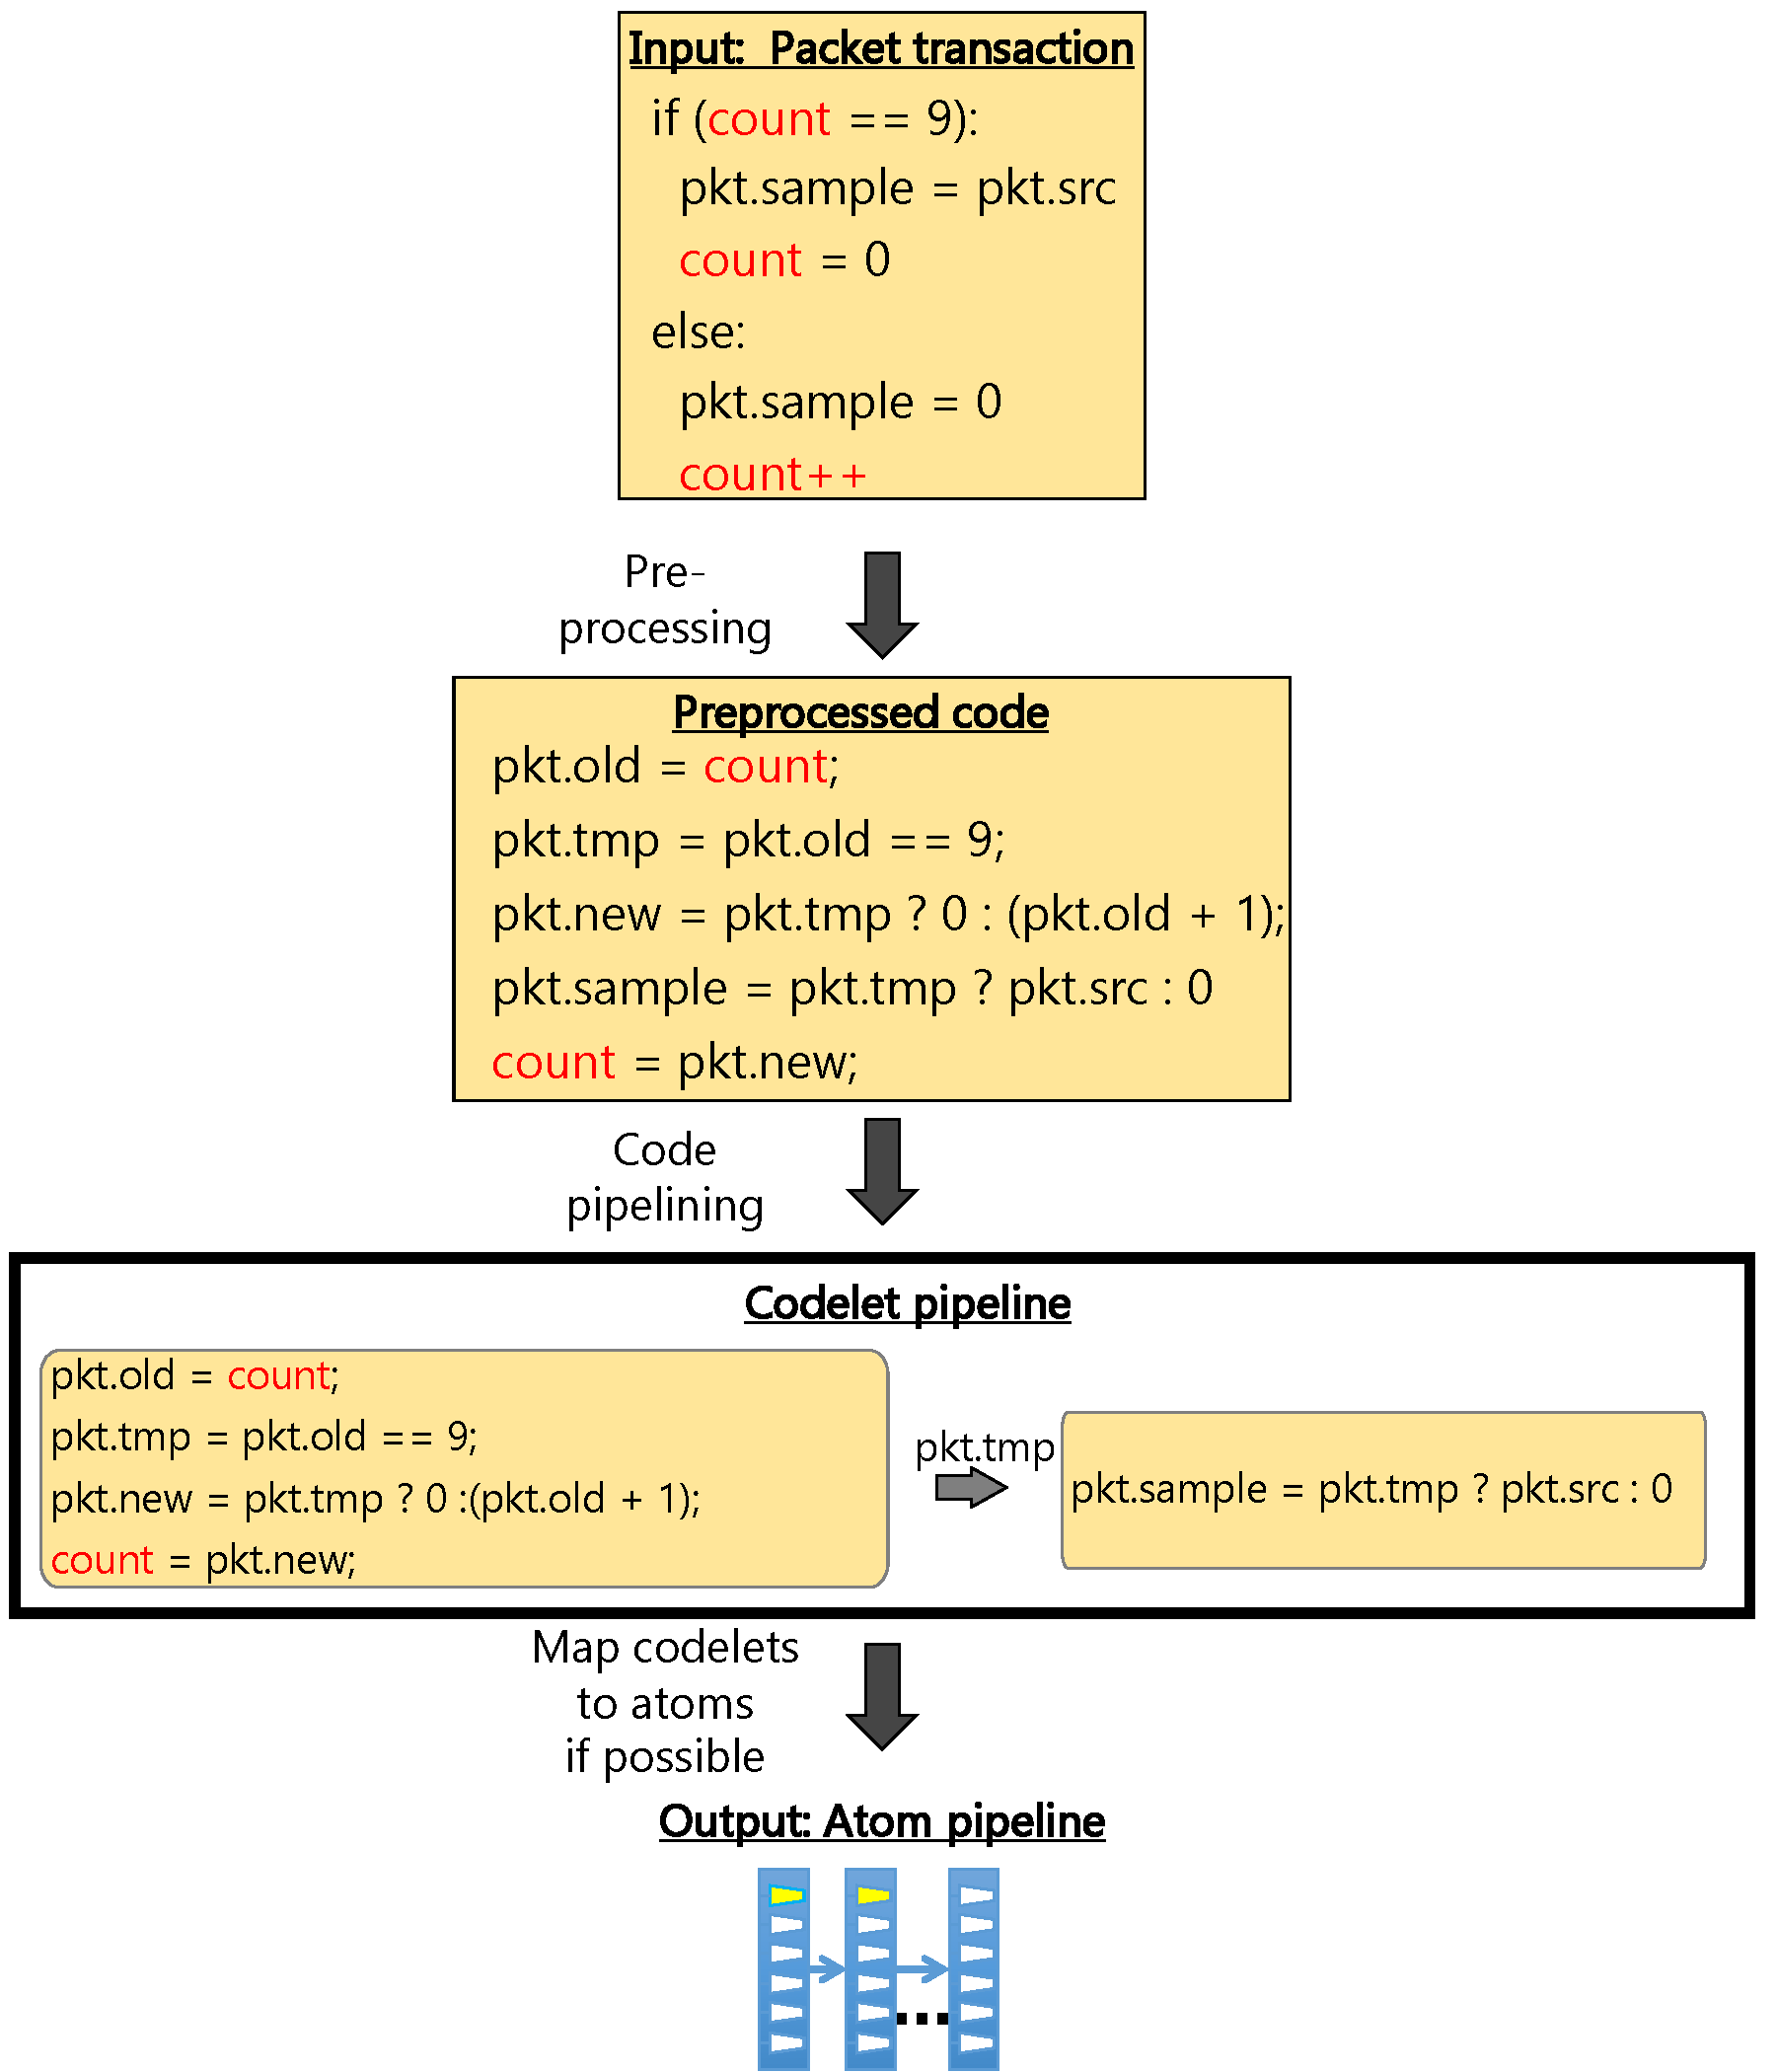
\includegraphics[width=\textwidth]{compiler_passes_example.pdf}
\caption{The three passes of Domino's compiler shown on the packet transaction
from Figure~\ref{fig:simple_transaction}.}
\label{fig:compiler_passes_example}
\end{figure}

The compiler has three passes (Figure~\ref{fig:compiler_passes_example}). First
(\S\ref{ss:preprocessing}), it preprocesses the code to make it easier to infer
dependencies between packet-processing operations. Second
(\S\ref{ss:pipelining}), the compiler transforms the preprocessed, but still
serial, packet transaction into a parallel pipeline of {\em codelets}.  When
pipelining, the compiler maintains the invariant that if each codelet executes
atomically and passes off its results to the next codelet, the behavior will be
indistinguishable from the packet transaction itself executing atomically on
each packet. Third (\S\ref{ss:code_gen}), the compiler maps each codelet
one-to-one to an atom provided by the underlying router, rejecting the code if
the codelet cannot be supported by the atom.

The compiler provides an {\em all-or-nothing} guarantee: if the compiler
compiles a program, the program will run at the line rate of the
router.\footnote{We use the term line rate in this dissertation to mean both
the maximum bit/packet rate of a particular router port/line (\eg 10 Gbit/s)
and the maximum aggregate bit/packet rate of a router: the product of the
per-port line rate and the number of ports (\eg 64 * 10 Gbit/s = 640 Gbit/s).
It should be clear from the context which interpretation of line rate we are
referring to. } All other programs that cannot run at the router's line rate
will be rejected. A program may be rejected either because the router's atoms
are not expressive enough for the program's operations or there aren't enough
atoms for all operations in the program. A conventional compiler for a
general-purpose CPU compiles all programs, but a program's run-time performance
depends on its complexity. In Domino, only programs that are simple enough to
run at the router's line rate will be compiled, obviating the need for any
performance profiling.

\subsection{Evaluation}
Developing atoms for a router is a chicken-and-egg problem. A router's atoms
determine what algorithms the router can support, while the algorithms
determine what atoms are required in the first place. Designing the right atoms
is especially important for a programmable router because, in contrast to a
general-purpose CPU, there is no way to ``emulate'' functionality in software
when hardware support is not available: recall that if an atom does not exist
to support a program's operations, the program will be rejected.

\begin{figure}
\centering
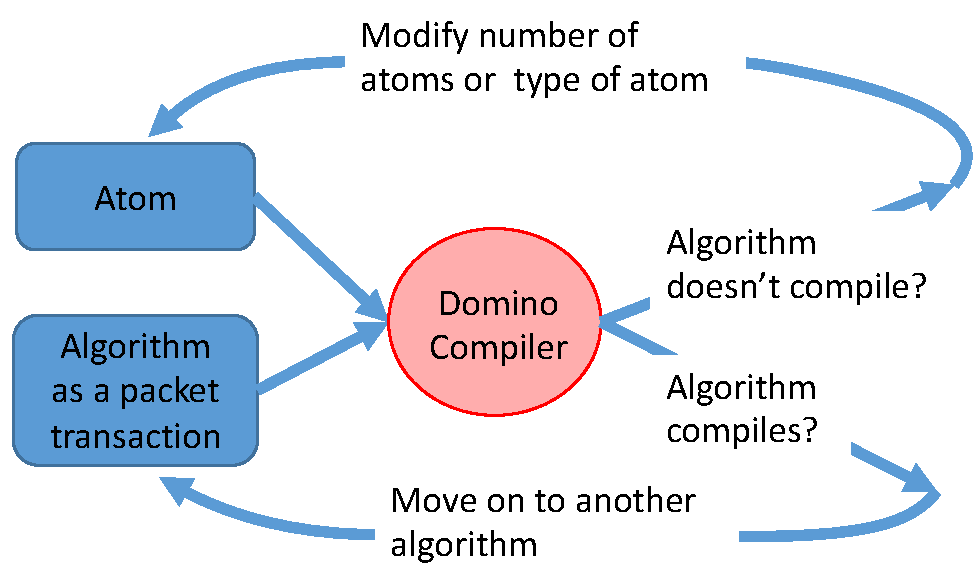
\includegraphics[width=0.5\columnwidth]{iterative_design_process.pdf}
\caption{Iterative atom design process}
\label{fig:iterative_design}
\end{figure}

To develop atoms, we use the Domino compiler to experiment with different atoms
and iteratively modify the atoms until they support enough algorithms
(Figure~\ref{fig:iterative_design}).  Using this process, we developed seven
atoms of increasing complexity (Table~\ref{tab:templates}) that allow us to
progressively program more and more algorithms from
Figure~\ref{fig:router_algos}. For instance, measurement using Bloom filters
only requires simple read and write operations on state. On the other hand,
heavy-hitter detection~\cite{opensketch} uses a count-min sketch~\cite{cormode}
that relies on an atomic counter. Finally, algorithms like flowlet
switching~\cite{flowlets} require conditional writes to a state variable.

After freezing the design of these atoms, we found that our atoms could express
several new use cases that were unanticipated when the atoms were designed
(Table~\ref{tab:atoms_generalize}). This provides us with some evidence that
these atoms are indeed programmable and can generalize to new algorithms beyond
the initial algorithms that influenced their design in the first place.

\section{Programmable packet scheduling}
Packet scheduling is an important determinant of network performance. The
choice of scheduling algorithm is tied to a network's performance goals. For
instance, an algorithm that divides link capacity fairly is ideal in a
multi-tenant setting~\cite{wfq}, while the shortest remaining processing time
algorithm is ideal for a single tenant who desires low flow completion
time~\cite{pFabric}. Today's routers provide a fixed set of scheduling
algorithms (\eg priority queues, Deficit Round Robin~\cite{drr}, and rate
limiting~\cite{tbf}). While configuration settings on these scheduling
algorithms can be tweaked, there is no way for an operator to program a new
scheduling algorithm that is tailored to their needs.

Routers lack programmable scheduling because there is no single abstraction to
express many scheduling algorithms~\cite{wfq, srpt, srr, pFabric, lstf} that
appear so different at first brush. This lack of a single unifying abstraction
is not merely an academic concern. It has practical consequences: in the
absence of a single abstraction that can then be hardened in hardware, we are
left with using a general-purpose substrate such as a CPU to program
scheduling. As we mentioned earlier, this can seriously hurt performance.

 Push In First Out Queues (PIFOs) (Chapter~\ref{chap:pifo}) provide such an
abstraction.\footnote{PIFOs were first used as a theoretical proof construct to
establish the equivalence of combined input-output queued routers and purely
output queued routers~\cite{pifo}. We show here that they can be used
practically for programmable packet scheduling.} They exploit our observation
that in many practical schedulers the relative order of packets that are
already buffered does not change in response to new packet arrivals
(\S\ref{s:deconstruct}). Hence, when a packet arrives, it can be pushed into
the right location based on a packet priority (push in), but packets are always
dequeued from the head (first out). A PIFO is simply a priority queue of
packets with a small program to assign each packet its priority.\footnote{We use
the term PIFO instead of priority queue because, within the context of
networking, priority queues typically refer to an implementation of
work-conserving priority scheduling. PIFOs can be used for both work-conserving
and non-work-conserving algorithms (\S\ref{s:expressive}).} Yet, by flexibly
programming a packet's priority assignment, a network operator can use PIFOs to
program a variety of previously proposed scheduling algorithms. 

\subsection{Programming model for packet scheduling} Our programming model for
scheduling couples a PIFO with a program to determine a packet's {\em rank} in
the PIFO. This rank can denote the packet's scheduling order (for
work-conserving algorithms such as Weighted Fair Queueing~\cite{wfq}) or
absolute wall-clock departure time (for non-work-conserving algorithms such as
traffic shaping~\cite{tbf}). This program is written as a packet transaction,
introduced earlier.  Depending on whether the program determines the scheduling
order or time, the program is called either a scheduling transaction or a
shaping transaction.

\begin{figure}
\begin{subfigure}[!h]{0.48\textwidth}
\vspace{0.4in}
\begin{lstlisting}[style=customcscriptsize]
f = flow(p) # compute flow from packet p
if f in last_finish:
 p.start = max(virtual_time, last_finish[f])
else: # p is first packet in f
 p.start = virtual_time
last_finish[f] = p.start + p.length/f.weight
p.rank = p.start
\end{lstlisting}
\caption{Scheduling transaction for the Start-Time Fair Queueing
implementation~\cite{stfq} of Weighted Fair Queueing.}
\label{fig:wfq_trans}
\hfill
\end{subfigure}
\begin{subfigure}[!h]{0.48\textwidth}
\begin{lstlisting}[style=customcscriptsize]
tokens = tokens + r * (now - last_time)
if (tokens > B):
  tokens = B
if (p.length <= tokens):
  p.send_time = now
else:
  p.send_time = now + (p.length - tokens) / r
tokens = tokens - p.length
last_time = now
p.rank = p.send_time
\end{lstlisting}
\caption{Shaping transaction for Token Bucket Shaping.}
\label{fig:tbf_trans}
\end{subfigure}
\vspace{-0.25in}
\caption{Examples of scheduling and shaping transactions. {\tt p.x} refers to a
packet field {\tt x} in packet {\tt p}.  {\tt y} refers to a state variable
that is persisted on the router across packets, \eg {\tt last\_finish} and {\tt
virtual\_time} in this snippet. {\tt p.rank} denotes the packet's computed
rank.}
\label{fig:example_transactions}
\end{figure}

A single PIFO coupled with a scheduling or shaping transaction can express many
classical scheduling algorithms, \eg Weighted Fair Queueing (Figure~\ref{fig:wfq_trans})
and Token Bucket Shaping (Figure~\ref{fig:tbf_trans}). But, a single PIFO is still restricted to
scheduling algorithms with the property that the relative order of packets that
are already buffered does not change in response to new packet arrivals. A
canonical class of scheduling algorithms that violate this relative order
property is the class of hierarchical scheduling algorithms. A well-known
example of this class is Hierarchical Packet Fair Queueing (HPFQ)~\cite{hpfq}.
HPFQ first divides up the link's capacity fairly among classes, and then when
each class is scheduled, divides up the class's transmission opportunities
fairly among its constituent flows. It can be thought of a recursive version of
fair queueing.

\begin{figure}[!t]
\centering
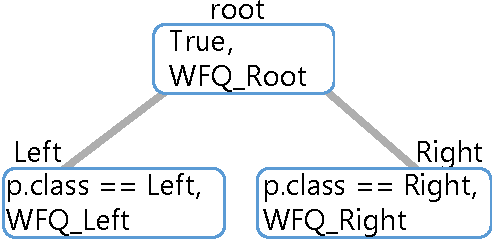
\includegraphics[width=0.5\textwidth]{pifo_hpfq_program.pdf}
\caption{Scheduling tree for HPFQ. The scheduling transactions WFQ\_Root,
WFQ\_Left, and WFQ\_Right are similar to Figure~\ref{fig:wfq_trans} and differ
only in how the flow is computed from the packet. This tree has no shaping
transaction.}
\label{fig:scheduling_tree}
\end{figure}

To support hierarchical scheduling, we extend our programming model from a
single PIFO to a tree of PIFOs. We also allow an entry in a PIFO to be either a
packet or a reference to another PIFO. More formally, a node in a {\em
scheduling tree} (Figure~\ref{fig:scheduling_tree}) has three attributes: (1) a
predicate that determines which packets are handled by that node, (2) a
scheduling transaction that determines a packet's rank in a scheduling PIFO
attached to that node, and (3) an optional shaping transaction that determines
a packet's rank in an optional shaping PIFO attached to that node. The shaping
transaction is optional because it is only relevant to non-work-conserving
schedulers. It can be disregarded entirely for work-conserving schedulers.

\begin{figure}[!t]
  \centering
  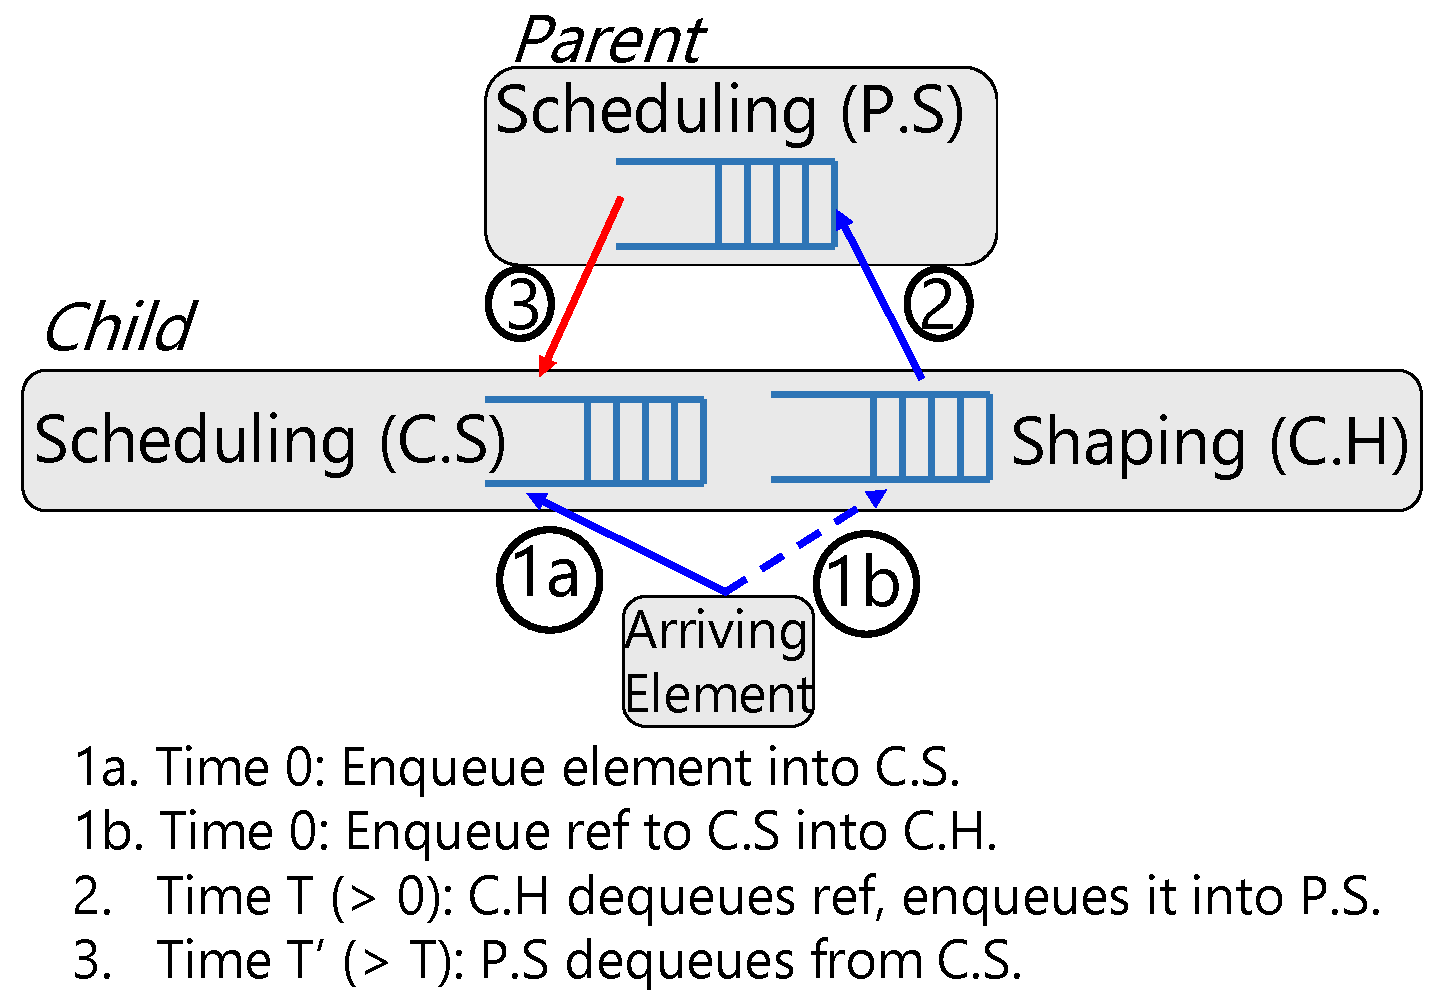
\includegraphics[width=0.6\columnwidth]{pifo_shaping_semantics.pdf}
  \caption{\textit{Child's} shaping transaction (1b) {\em defers} enqueue
  into \textit{Parent's} scheduling PIFO (2) until time T.  Blue arrows
  show enqueue paths. Red arrows show dequeue paths.  }
  \label{fig:shaping_timing}
\end{figure}

We now explain the semantics of a scheduling tree during dequeues and enqueues.
During a dequeue, we walk the scheduling tree starting from the root. We
dequeue the scheduling PIFO at the root, resulting in either a reference to
another scheduling PIFO or a packet. If the result is a packet, we are done,
and we transmit the packet. If not, we continue recursively, dequeueing from
the scheduling PIFO that is pointed to until we find a packet.

When a packet is enqueued, we walk the tree from the leaf whose predicate
captures the packet to the root. Along this leaf-to-root path, we execute
scheduling and (optionally) shaping transactions attached to the path's nodes.
Figure~\ref{fig:shaping_timing} illustrates the timing of various operations
related to a node's scheduling and a shaping PIFO. A node's scheduling
transaction inserts either a packet or a PIFO reference into the node's
scheduling PIFO. A node's shaping transaction inserts a reference $R$ to the
node's scheduling PIFO in the node's shaping PIFO. Once the shaping transaction
has executed, execution of transactions for this packet is temporarily
suspended.  When the reference $R$ is dequeued from the shaping PIFO, it is
enqueued into the node's parent's scheduling PIFO using the parent's scheduling
transaction and the rest of the leaf-to-root path is resumed.  The shaping PIFO
thus provides an optional mechanism for a node to {\em defer} enqueues into its
parent's scheduling PIFO, which is useful when combining hierarchical
scheduling with traffic shaping (Figure~\ref{fig:hshaping} in
Chapter~\ref{chap:pifo} shows an example.).

\subsection{Expressiveness of our programming model}

The PIFO-based programming model unifies several scheduling algorithms and
allows us to program a wide variety of scheduling algorithms using the single
PIFO primitive, \eg Weighted Fair Queueing~\cite{wfq}, Token Bucket
Shaping~\cite{tbf}, Hierarchical Packet Fair Queueing~\cite{hpfq}, Least-Slack
Time-First~\cite{lstf}, the Rate-Controlled Service Disciplines~\cite{rcsd},
and fine-grained priority scheduling (\eg Shortest Job First).

\subsection{Hardware for programmable scheduling}
\label{ss:intro_pifo_hardware}

We designed high-speed hardware to support a PIFO-based programming model. When
designing hardware for PIFOs, we set out to meet performance targets that are
typical for a single-chip shared-memory router today. These are routers that
are built out of a single chip (also called an application-specific integrated
circuit or ASIC), and whose packet buffer and scheduling logic is shared across
all ports. Sharing the packet buffer and scheduling logic reduces the memory
and digital logic cost associated with packet scheduling.

For concreteness, we picked a target clock frequency of 1 GHz to reflect the
requirement of performing one enqueue and one dequeue every nanosecond, typical
of high-speed routers today~\cite{rmt}. We targeted a packet buffer of size 12
MByte based on the buffer size of the Broadcom Trident II~\cite{bcom_buffer}, a
commercial single-chip shared-memory router. With a cell size of 200
bytes,\footnote{A cell is the minimum unit of memory allocation in the packet
buffer.} a 12 MByte buffer can support up to 60000 packets in the worst case.

Hence we need a PIFO that can support up to 60K packets. A naive way to
implement a 60K-entry PIFO is to use a flat sorted array of 60K elements and
insert an incoming element into this array in a manner reminiscent of insertion
sort. Concretely, an incoming element's rank would be compared in parallel to
the ranks of all 60K elements. This would produce a bitmask denoting which
elements were greater than or lesser than the incoming element.  Because the
array is always sorted, the bitmask would have a single 0-to-1 transition.  The
position of this 0-to-1 transition could be detected using a priority encoder.
Finally, the new element could be inserted into this position.  However, the
difficulty with this approach is that it is hard to lay out 60K parallel
comparators, one for each element in the PIFO.

Instead, we exploit the observation that in most practical scheduling
algorithms, scheduling is performed across flows and not individual packets.
This is because, in most schedulers, packet ranks increase monotonically across
consecutive packets within a flow. This ensures that packets within a flow are
transmitted in the order in which they arrive, thereby preventing packet
reordering within a flow.

Because ranks increase monotonically within a
flow, we only need to look at the first packet of each flow to determine which
packet to dequeue next. This reduces the number of elements that need to be
sorted from 60K packets in the naive implementation to around 1K flows in the
smarter implementation. We picked this 1K number with reference to the Broadcom
Trident II that supports \textasciitilde10 queues on each of its
\textasciitilde100 ports.

We find that transistor technology has evolved to the point where it is
relatively cheap to build a sorted array of 1K flows, where a flow can be
enqueued into or dequeued from the array every nanosecond. In a recent
industry-standard 16 nm technology node, a hardware design for a programmable
5-level hierarchical scheduler costs less than 4\% additional chip area
relative to a 200 \si{\milli\meter\squared} baseline router
chip~\cite{glen_parsing}.

\section{Scalable network measurement}
Chapter~\ref{chap:perf_query} considers the problem of programmable and
scalable network measurement. Concretely, can we allow network operators to
flexibly specify the per-flow statistics they want to measure (\eg a moving
average over queueing latencies or a count of packets or bytes) at the flow
granularity they desire (\eg at the 5-tuple level or at the level of each
distinct destination IP address)? Current router solutions for
measurement~\cite{netflow, tetration-telemetry} fix either the statistics that
can be measured or the granularity at which the statistics can be measured. The
challenge here is to provide a set of measurement primitives that can cover a
range of statistics while also scaling to a large number of flows, because the
granularity of a flow can be as fine-grained as the 5-tuple.

\begin{figure}
\begin{minipage}[!h]{\textwidth}
\centering
\begin{lstlisting}
result = filter((*\pktlog,*) qid == Q && tout - tin > 1ms)
// Filter out packets whose queueing delay at queue Q exceeds one ms.
\end{lstlisting}
\end{minipage}

\begin{minipage}[!h]{\textwidth}
\centering
\begin{lstlisting}
result = map((*\pktlog,*) [tin/epoch_size], [epoch])
// Round off packet time stamps to the nearest epoch.
\end{lstlisting}
\end{minipage}

\begin{minipage}[!h]{\textwidth}
\begin{lstlisting}
def count([c], []):
  c = c + 1
result = groupby((*\pktlog{}*), [(*\codeftuple{}*)], count)
// Partition packets by 5-tuple and count the number of packets in each 5-tuple.
\end{lstlisting}
\end{minipage}
\caption{Three example \TheSystem queries. {\ct \pktlog{}} refers to the
original packet performance stream with one tuple for each packet seen in the
network.}
\label{fig:example_queries}
\end{figure}

\subsection{Programming model} To allow network operators to express a wide
range of performance measurement questions, we provide them with the
abstraction of a single performance packet stream for the entire network.
Conceptually, the performance packet stream is a stream of tuples, one for each
packet, containing information identifying the packet (source and destination
address and ports) and its performance information (the timestamp at which the
packet was enqueued into and dequeued from each queue in the network).

Network operators can write queries that operate on this performance packet
stream using a query language called \TheSystem. \TheSystem has functional
constructs like {\ct map}, {\ct filter}, and {\ct groupby} similar to
functional APIs in programming languages like Python, Java, Scala, and Haskell.
Figure~\ref{fig:example_queries} shows some example queries in \TheSystem.
These constructs take a stream of tuples as input and return an output stream
of tuples. Because all constructs produce and consume streams, \TheSystem
queries can be easily composed.

The output stream either transforms each tuple in the input stream ({\ct map}),
drops certain tuples from the input stream based on a predicate ({\ct filter}),
or partitions the input stream into substreams based on a predicate and then
aggregates the tuples within each substream based on a user-defined aggregation
function ({\ct groupby}). \TheSystem's use of user-defined aggregation
functions differentiates its groupby construct from the groupby construct
supported by classical query languages like SQL. SQL only supports specific
order-independent aggregation functions like counts and averages. SQL does not
allow general, user-defined, and potentially order-dependent aggregation
functions. 

\subsection{Hardware for programmable network measurement}
\label{ss:intro_pq_hardware}

A naive implementation of performance queries would stream every packet to a
centralized collection server, which would execute the performance query on the
incoming packet stream. However, this would require enormous computational
capacity on the server and a separate measurement network just to stream every
packet to the server. For instance, modern stream processing systems support a
throughput of \textasciitilde100K--1M operations per second per
core~\cite{kafka_benchmark, redis_benchmark, memcached_benchmark,
redis_vs_memcached_update, spark-streaming}, but processing every single packet
from a single 1 Tbit/s router requires around \textasciitilde100M operations
per second even for relatively large 10000 bit packets. Instead, we use programmable
routers as first-class citizens to perform early filtering, aggregation, and
packet transformations. The net effect is a substantial reduction in the amount
of data sent out to and processed by the collection server.

Many of Marple's constructs (\eg {\ct map} and {\ct filter}) are {\em
stateless} in the sense that they do not need to maintain any router state. For
instance, a {\ct map} query could take an input packet stream, round
off the enqueue timestamp of each packet in the stream to the nearest
millisecond, and return the result as a new stream.  This query is stateless
because it can operate independently on each packet without maintaining any
state on the router that persists between packets. Supporting stateless queries
 is relatively straightforward. Emerging
programmable router chips~\cite{rmt, xpliant, flexpipe, tofino} already provide
an instruction set that performs stateless transformations on packet headers.
We leverage this instruction set as is to execute stateless queries because a
packet-processing pipeline naturally fits the streaming model of our queries.

On the other hand, the {\ct groupby} query is {\em stateful}. To see why,
consider a {\ct groupy} query that (1) partitions the packet stream into
substreams based on the 5-tuple and (2) counts the number of packets within
each substream. This query is stateful because it needs to maintain a
dictionary mapping each 5-tuple to its count as part of the persistent router
state. To implement the {\ct groubpy} query, this dictionary is updated by
incrementing some 5-tuple's counter on each packet. To support \TheSystem's
stateful construct, the {\ct groupby}, we design a programmable key-value store
in hardware. The keys represent the flows and the values represent the state
being aggregated according to the aggregation function as packets are
processed. In the example above, the key would be a 5-tuple and the value would
be a count of packets belonging to that 5-tuple.

This key-value store has two requirements that are at odds with each other: it
needs to be fast to process packets at the router's line rate (a packet every
nanosecond), and it needs to be large to store a large number of flows. Static
random-access memory (SRAM) can be accessed once every nanosecond, but has low
memory density and can only fit a small number of flows. On the other hand,
dynamic random-access memory (DRAM) has much better density allowing it to
support many more flows, but can be accessed only once every ten nanoseconds or
so.

We use caching to address both requirements: a fast SRAM cache stores the
currently active flows, while a backing store in DRAM handles evictions from
the cache. However, cache misses in traditional processor designs lead to
unpredictable memory access latencies while the data is being fetched from the
main memory. A processor handles this by occasionally stalling its pipeline to
handle a cache miss. But stalling a router pipeline prevents us from providing
the deterministic latency guarantees that routers are known and benchmarked
for.

\begin{figure}
\centering
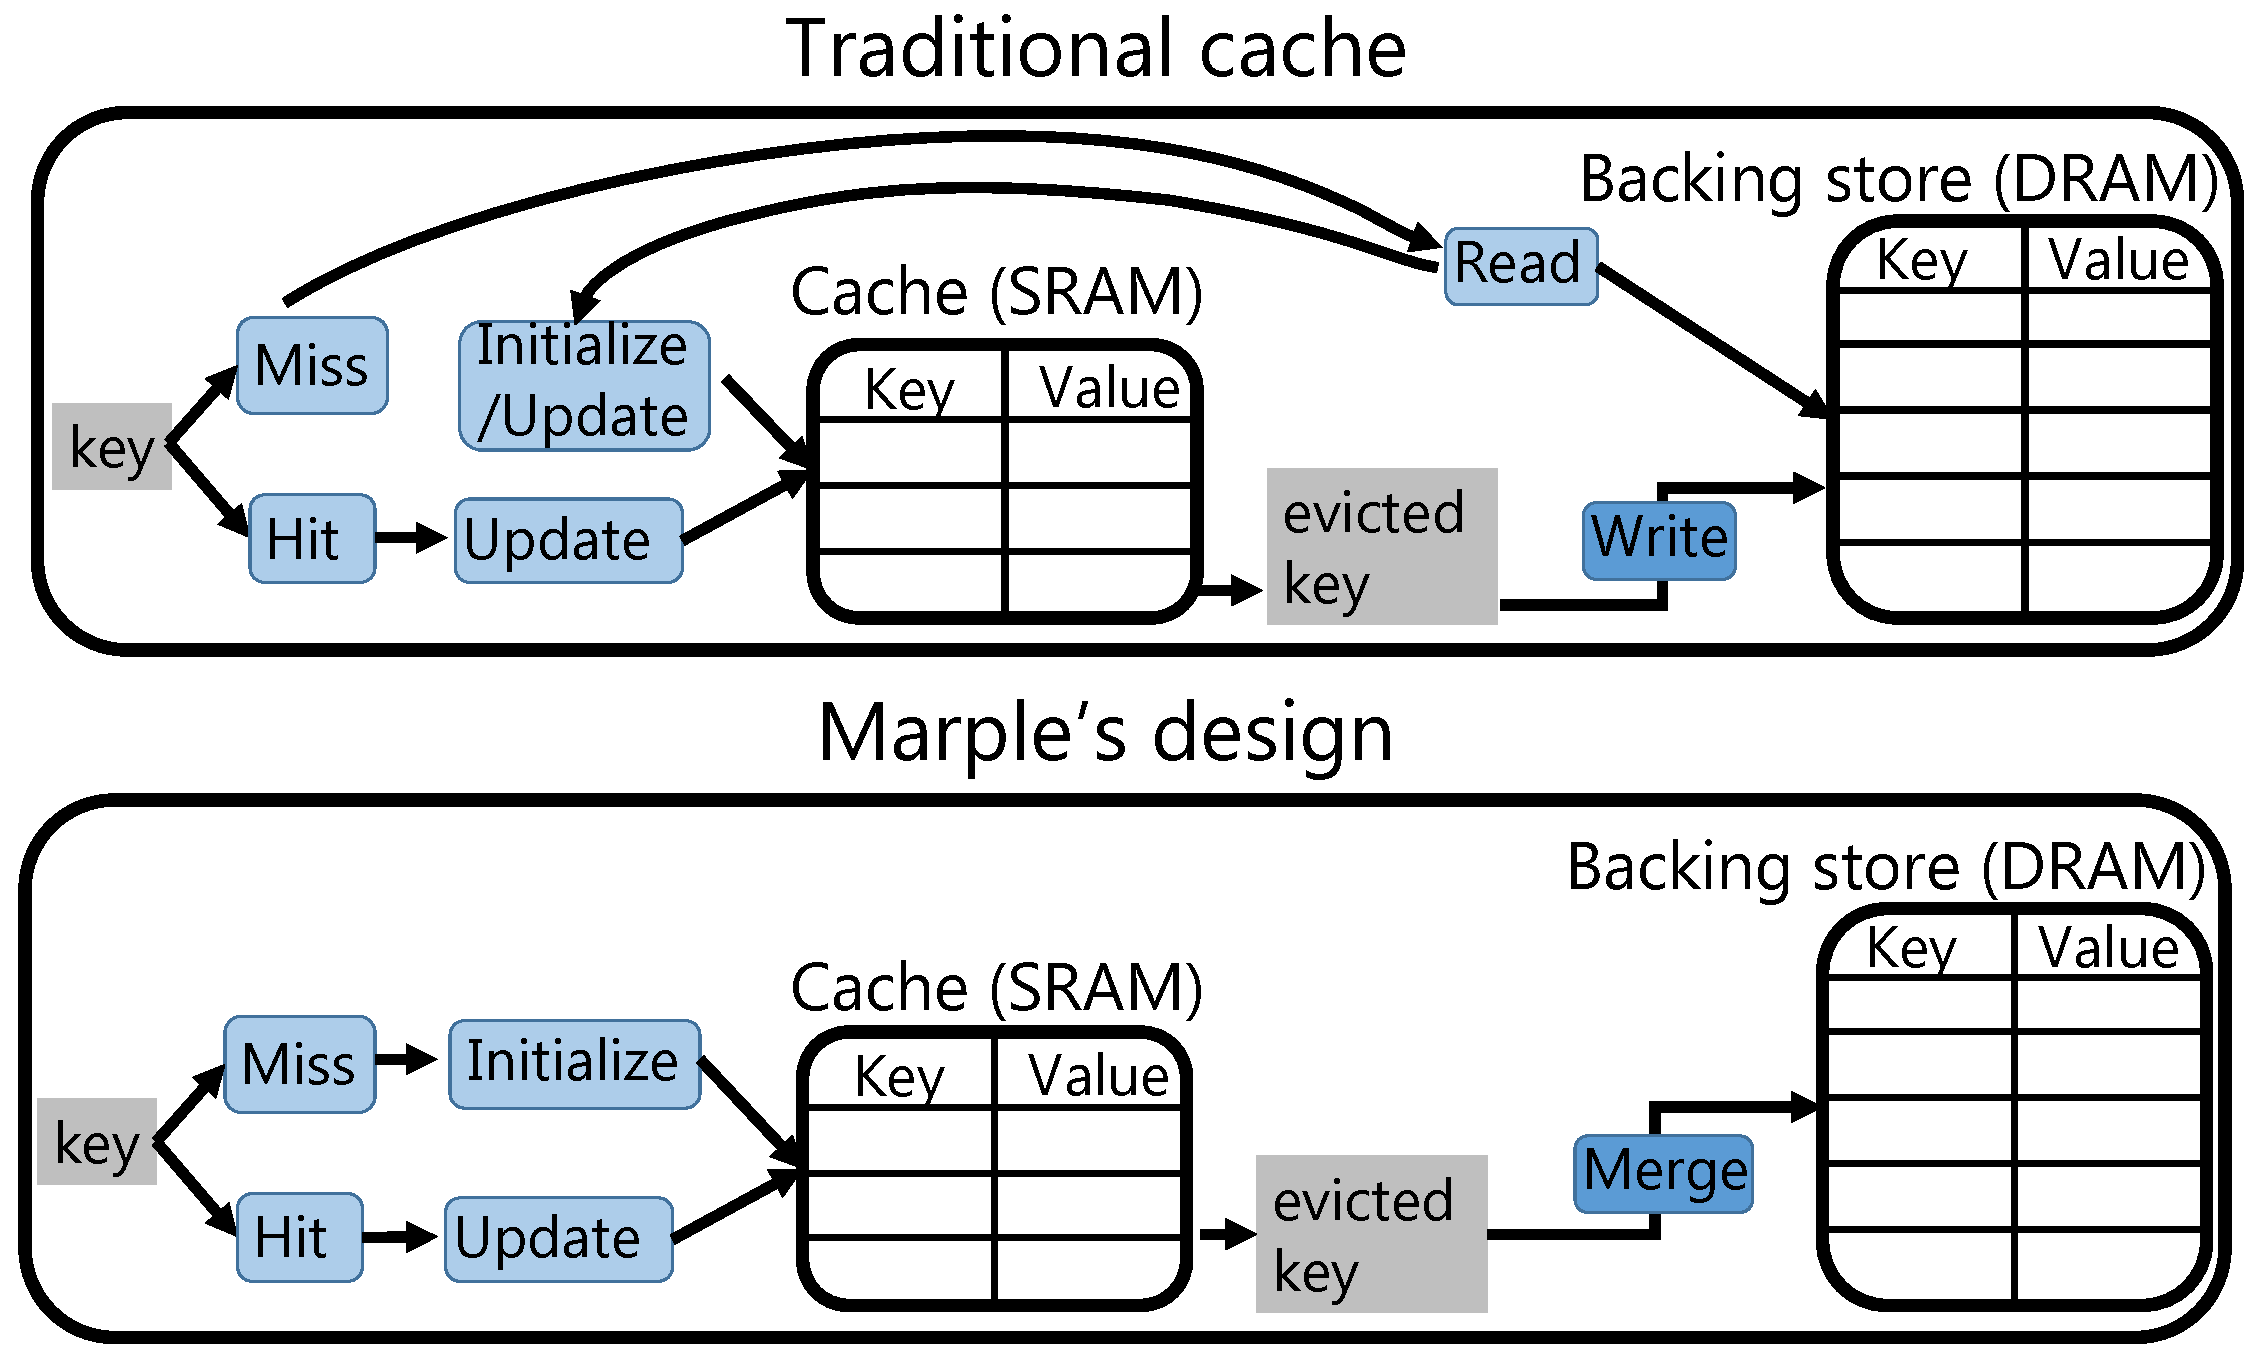
\includegraphics[width=0.6\columnwidth]{pq_kv_store.pdf}
\caption{\TheSystem's key-value store vs. a traditional cache}
\label{fig:hw_diff}
\end{figure}

Instead, as Figure~\ref{fig:hw_diff} shows, we treat a cache miss as the
arrival of a packet from a new flow and initialize the cache entry as though we
have just started aggregating packets from a new flow. When this cache entry is
eventually evicted, we {\em merge} it against the old value for that entry in the
backing store. The merge operation requires reading and writing from DRAM, which does
incur unpredictable access latencies. But, it happens off the critical path
during evictions alone. Importantly, it does not affect the critical path of
packet processing in the router's chip.

What exactly does this merge operation look like? As a simple example, if the
value in the key-value store was a counter; the merge operation would then
simply add up the old and new counts.  But is it always possible to merge an
aggregation function accurately \ie the value after the merge should be the
same as the value that would be obtained in an ideal system with an infinitely
large cache that needs no merging?

We can prove (\S\ref{ss:proofs}) that there are aggregation functions for which
it is not possible to merge efficiently without losing accuracy. However, we
formally characterize a class of aggregation functions for which such merging
{\em is} possible without losing accuracy. We call this class the class the
{\em linear-in-state} class because aggregation functions in this class take
the following form:
\begin{equation}
S = A(p) * S + B(p)
\end{equation}
Here $S$ is the state/value that is being updated by the aggregation function,
while $A$ and $B$ are functions of a a bounded number of packets into the past
including the current one. The linear-in-state class captures a variety of
aggregation functions including counters, predicated counters, moving average
filters, and arbitrary functions on sliding windows.

\subsection{Evaluation} We evaluate \TheSystem's expressive power by using it
to express several diverse performance queries, \eg tracking the loss rate on a
per-flow basis, measuring the extent of reordering in a TCP flow, measuring a
moving average of queueing latencies on a per-flow basis, and detecting the
presence of TCP incast.

Our \TheSystem compiler compiles queries to two different targets: an atom
pipeline to determine the hardware feasibility of \TheSystem queries and a
P4-based software router~\cite{p4-bmv2} for end-to-end case studies of
\TheSystem in Mininet~\cite{mininet}. We find that \TheSystem queries occupy a
small fraction of the router's computational and memory resources.
Computationally, queries require a small number of atoms. Memory-wise, the
programmable key-value store requires an SRAM cache that occupies a modest
amount of additional chip area. Our Mininet experiments show that \TheSystem
can be used to iteratively troubleshoot problems such as occasional latency
spikes that occur because of bursty background traffic.

 We determine the eviction rate from the SRAM cache using a trace-driven
simulation on publicly available packet traces from CAIDA~\cite{caida2016,
caida2014} and a university data center~\cite{theo_dc}. For a 64 Mbit on-chip
cache, which occupies about 10\% of the area of a 64×10-Gbit/s router chip, we
estimate that the cache eviction rate from a single top-of-rack router can be
handled by a single 8-core server running Redis~\cite{redis}. Relative to a
strawman that sends every packet to the collection server (\ie a 100\% eviction
rate), the on-chip cache results in a reduction in eviction rate of 34--81x
(Figure~\ref{fig:evt-rate-queries}).

\section{Lessons learned} We conclude this chapter by distilling some general
lessons for designing fast and programmable routers in the future that go
beyond the specific contributions of each of the three systems.

\subsection{The power of specialization} The most important lesson here is the
power of specialization: the idea of targeting hardware and software to
specific classes of router functionality.  The three systems in the
dissertation demonstrate how narrowing our focus to specific router
functionality allows us to resolve the performance-programmability tradeoff
that has affected software routers so far. Put differently, it allows us to get
the best of both worlds, but for restricted classes of router functionalities.

More formally, the three systems are specialized in the sense that they are not
Turing-complete: they cannot simulate a Turing machine, an idealization of the
general-purpose CPU.  We refer the reader to \S\ref{domino_ss:limitations} and
Table~\ref{tab:restrict}, \S\ref{pifo_ss:limitations}, and \S\ref{sec:compiler}
for specific examples of what each of the three systems cannot express.

Yet, each covers a large number of use cases within specific functionality
classes (stateful data-plane algorithms, scheduling, and measurement queries)
without giving up performance relative to a fixed-function router. Viewed
differently, by specializing, each system provides an order of magnitude
improvement in performance relative to a general-purpose software router.
Intellectually, these results suggest that there is a rich space of system
designs that is as yet unexplored---if we choose to look beyond Turing-complete
systems. 

\subsection{Jointly designing hardware and software} We are entering an era
where Moore's law has slowed down or effectively stopped~\cite{dark_silicon,
four_horsemen}.  In this new era, transistors are no longer guaranteed to get
smaller or faster every year. Besides, it may not be cost effective to move to
smaller or faster transistors because of rising non-recurrent engineering costs
associated with newer transistor technologies~\cite{nre_moonwalk}. In the
heyday of Moore's law, processor hardware automatically got faster year on
year. Software automatically enjoyed the free lunch of improved performance
because of improvements in the underlying hardware. With the imminent end of
Moore's law, it is no longer apparent how these performance improvements will
be sustained.

Jointly designing hardware and software in service of a higher level goal
suggests a way to continue improving performance. Year on year, the greatest
performance improvements could now come from human creativity in specializing
hardware to specific goals and then appropriately exposing this specialized
hardware to software. This is already visible in domains such as machine
learning. For instance, the tensor processing unit~\cite{tpu} is a chip
tailored to deep learning, and TensorFlow~\cite{tensorflow} is its
corresponding programming model.

The systems presented in this dissertation are examples of joint hardware and
software design in the context of networking, where we develop both the
underlying hardware (atoms, PIFOs, and hardware key-value stores) and the
corresponding software (packet transactions, scheduling trees, and performance
queries) for specific goals (stateful data-plane algorithms, scheduling, and
statistics measurement).

\section{Source code availability}
Source code for the systems presented in this dissertation is available online
at \url{http://web.mit.edu/domino}, \url{http://web.mit.edu/pifo}, and
\url{http://web.mit.edu/marple}. Each URL contains links to the relevant source code for each project:
\begin{CompactEnumerate}
\item For Domino, the source code consists of a C++ simulator for high-speed router hardware (\url{https://github.com/packet-transactions/banzai}), C++ code for the Domino compiler (\url{https://github.com/packet-transactions/domino-compiler}), Domino code (\url{https://github.com/packet-transactions/domino-examples}) for the algorithms described in Tables~\ref{tab:algorithms} and \ref{tab:atoms_generalize}, and Verilog code for the atoms (\url{https://github.com/packet-transactions/atomsyn}).
\item For PIFO, the source code consists of a C++ reference implementation of the PIFO hardware (\url{https://github.com/programmable-scheduling/pifo-machine}), and a Verilog implementation of the PIFO hardware (\url{https://github.com/programmable-scheduling/pifo-hardware}).
\item For Marple, the source code consists of a Java compiler for Marple queries (\url{https://github.com/performance-queries/marple}), instructions to setup a testbed for Mininet experiments using Marple (\url{https://github.com/performance-queries/testbed}), and the example Marple queries used in our evaluation (\url{https://github.com/performance-queries/marple-domino-experiments}).
\end{CompactEnumerate}


%%
%%\subsection{Vertically integrated thinking} Philosophically, the results in the
%%dissertation advocate for vertically integrated thinking, where a single system
%%design incorporates the entire computing stack. We design programmable hardware
%%at the bottom of this stack, work our way up through the compiler for this
%%hardware, and expose this to the programmer at the highest layer through a
%%domain-specific language.
%%
%%For decades now, systems programmers have treated the hardware as programmable,
%%but unmodifiable. There are undeniable benefits to writing software for
%%off-the-shelf commodity hardware because it is immediately deployable. This is
%%in contrast to vertically integrated systems that need to be first designed in
%%hardware and then programmed in software. At the same time, the results here
%%suggest that there are substantial performance benefits from redesigning the
%%entire stack from the ground up.
